\documentclass[10pt]{beamer}

% Paquetes
\usepackage[T1]{fontenc}    % Para escribir en español
\usepackage[spanish]{babel}    % Para escribir en español
\usepackage{hyperref}    % Para hacer links a la web
\usepackage{listings}    % Para incluir código

% Setup imagenes
\graphicspath{ {out/}}

% Estilos
\usetheme{Madrid}


% Personalización del footer
\setbeamertemplate{footline}{%
  \leavevmode%

  \hbox{\begin{beamercolorbox}[wd=.5\paperwidth, center, ht=2.5ex]{author in head/foot}%
    \usebeamerfont{author in head/foot}\insertshortauthor%
  \end{beamercolorbox}%

  \begin{beamercolorbox}[wd=.4\paperwidth, center, ht=2.5ex]{title in head/foot}%
    \usebeamerfont{title in head/foot}\insertshorttitle%
  \end{beamercolorbox}%

  \begin{beamercolorbox}[wd=.1\paperwidth, center, ht=2.25ex]{date in head/foot}%
    \insertframenumber{} / 15%%
  \end{beamercolorbox}
  }%

  \vskip0pt%
}%

% Eliminar barra de navegación
\beamertemplatenavigationsymbolsempty


% Info para la title page
\title{Concurrencia a Museos de Argentina}
\subtitle{Relación con otros consumos culturales}
\author{Nazareno Magallanes \and Javier Spina \and Lautaro Terreno}
\institute[ECyT]
{
  {\large Introducción a la Ciencia de Datos}
  \and
  Escuela de Ciencia y Tecnología
  \and
  Universidad Nacional de San Martín
}
\date{14 Noviembre 2022}


% Inicio del documento
\begin{document}


\frame{\titlepage}


% Pregunta y contexto
\begin{frame}
  \frametitle{La pregunta y su contexto}

  \begin{block}{La pregunta}
    ¿Cómo aumentar la concurrencia a los museos?
  \end{block}

  \vfill

  \begin{center}
    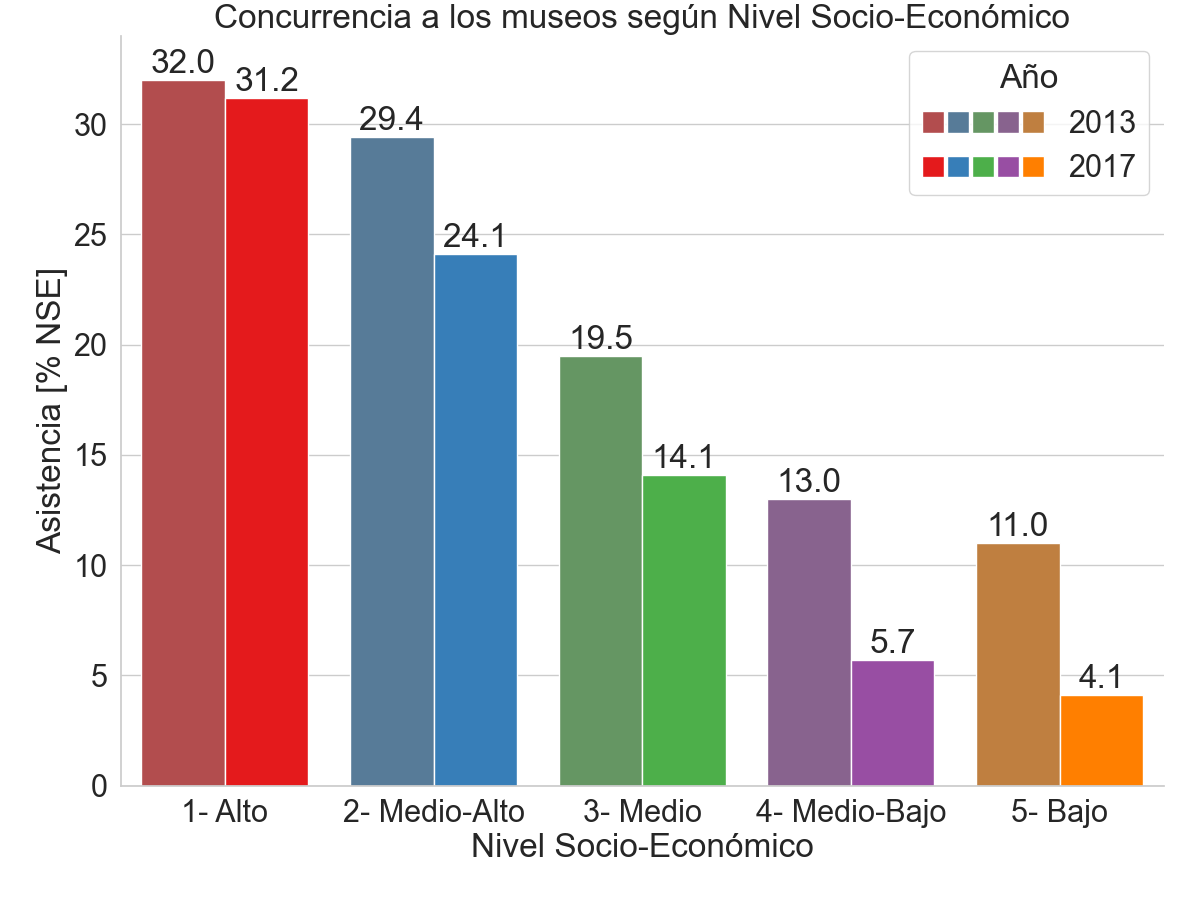
\includegraphics[height=0.6\textheight]{asist_museo_nse_x100}
  \end{center}
\end{frame}


% Presentación
\begin{frame}
  \frametitle{Presentación del \textit{dataset}}

  \begin{columns}
    \column{0.5\textwidth}
      \begin{center}
        
\includegraphics[height=0.7\textheight]{encc_informe_portada.pdf}
      \end{center}

    \column{0.5\textwidth}
      \begin{itemize}
        \item Se trabajó con el \textit{dataset} asociado a la \textbf{Encuesta Nacional de Consumos Culturales} realizada en 2017. 
        \item Se complementó con datos abiertos de los Museos de Argentina y un Shapefile de Argentina de las 23 provincias y CABA.
      \end{itemize}
  \end{columns}
\end{frame}


% Limpieza de datos
\begin{frame}
  \frametitle{Trabajo inicial: unidades y variables}

  \begin{columns}
    \column{0.2\textwidth}
      Encuesta\\
      2802 unidades\\
      450 variables

    \column{0.5\textwidth}
      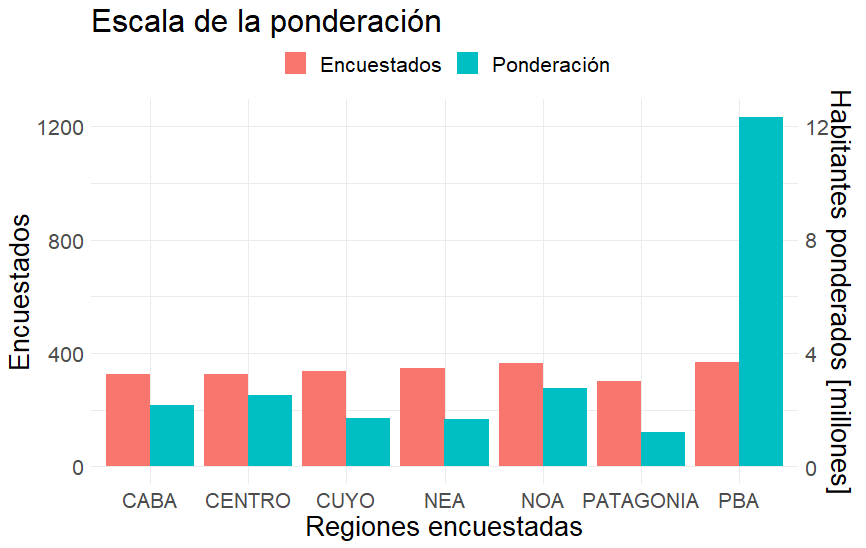
\includegraphics[width=\textwidth]{pondera}

    \column{0.3\textwidth}
      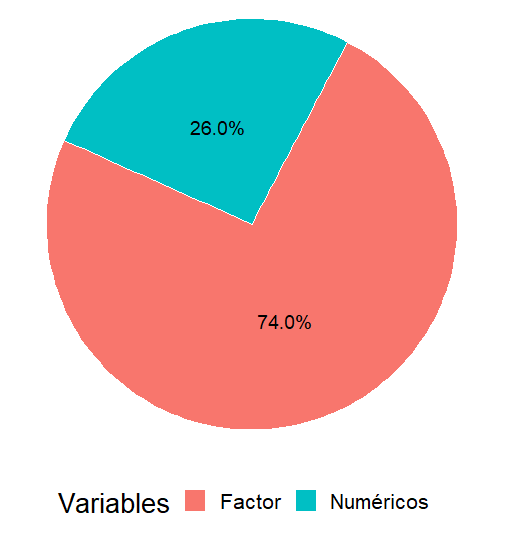
\includegraphics[width=0.8\textwidth]{tipos_variables}
  \end{columns}

  \vfill

  \begin{columns}
    \column{0.2\textwidth}
      Museos\\
      1182 unidades\\
      27 variables

    \column{0.3\textwidth}
      \resizebox{\textwidth}{!}{%
        \begin{tabular}{|l|c|}
          \hline
          Localizacion & Unidades\\ \hline
          Precisa & 1179 \\ \hline
          Centroide de la localidad & 1 \\ \hline
          Centroide por proximidad & 2\\ \hline
        \end{tabular}
      }

      \column{0.45\textwidth}
        \begin{itemize}
          \item Se agregó la columna región en el \emph{dataset} de la ubicación de los museos.
          \item Se limitó el Shapefile de Argentina a la vista continental.
        \end{itemize}
  \end{columns}
\end{frame}


% Hipótesis
\begin{frame}
  \frametitle{Hipótesis de trabajo}
  Se trabajó alrededor de dos hipótesis para aumentar la concurrencia.

  \begin{block}{Hipótesis 1}
    Instalar nuevos museos aumentará la concurrencia a los mismos.
  \end{block}

  \begin{block}{Hipótesis 2}
    Hacer más atractivas las propuestas de los museos en base a los otros consumos culturales aumentará la concurrencia.
  \end{block}
\end{frame}


% Análisis 1
\begin{frame}
  \frametitle{Análisis Exploratorio}

  \begin{columns}
    \column{0.5\textwidth}
      \begin{figure}
        \vspace{-2.75em}
        \includegraphics[width=\textwidth]{museos_datosabiertos.png}
      \end{figure}
    
    \column{0.5\textwidth}
      \begin{figure}
        \vspace{-1.5em}
        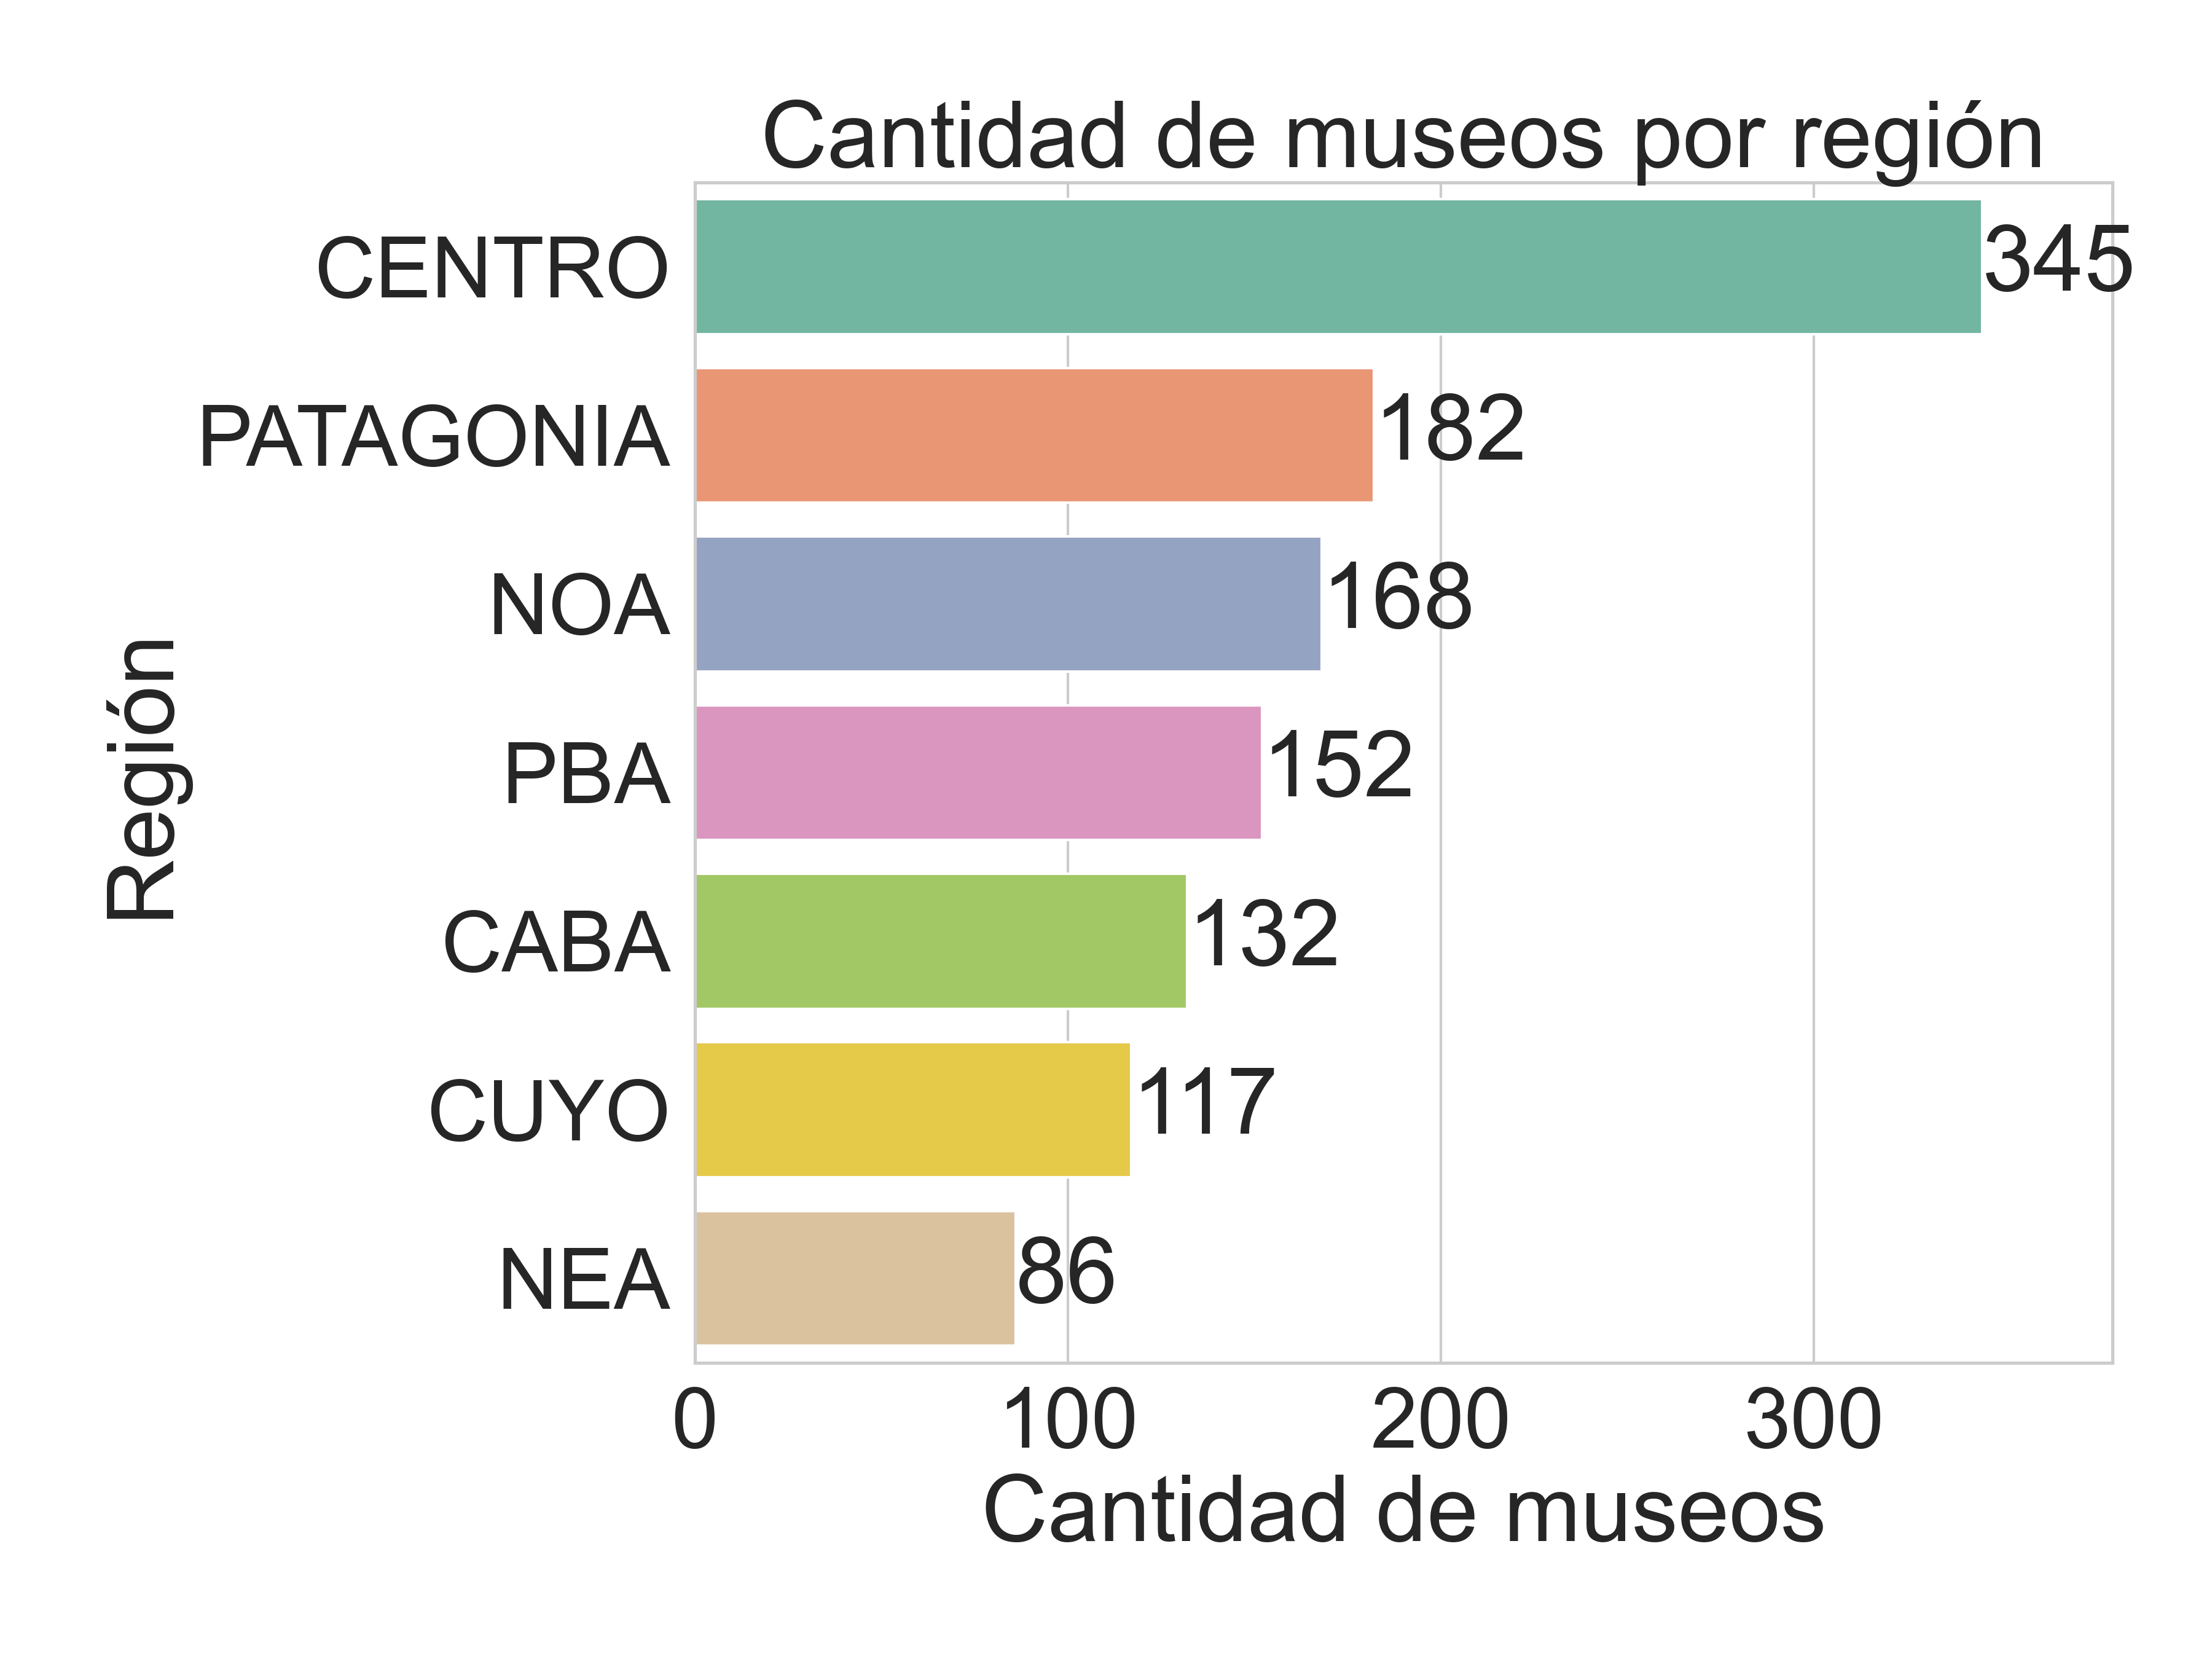
\includegraphics[width=0.9\textwidth]{cantidad_museos.png}
      \end{figure}

      \begin{figure}
        \vspace{-2.25em}
        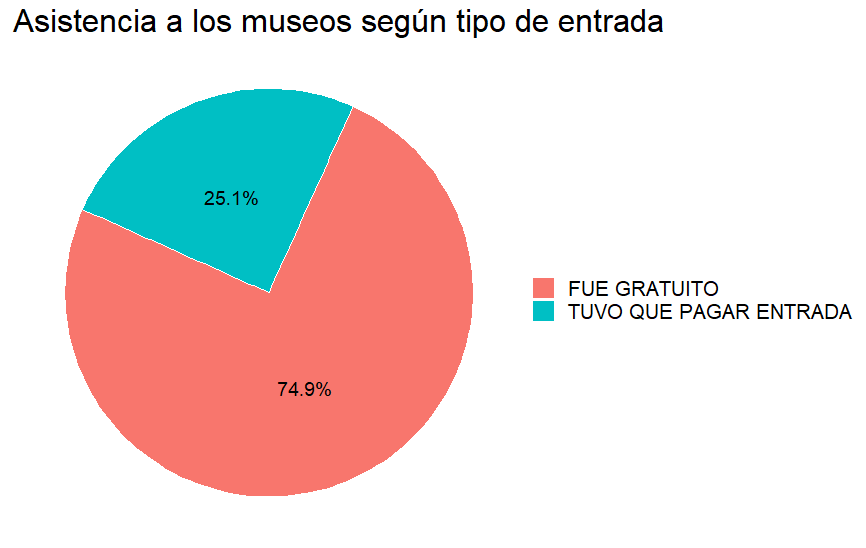
\includegraphics[width=0.9\textwidth]{entradas.png}
      \end{figure}
  \end{columns}
\end{frame}


% Cantidad de entradas
\begin{frame}
  \frametitle{Visitas a los museos}

    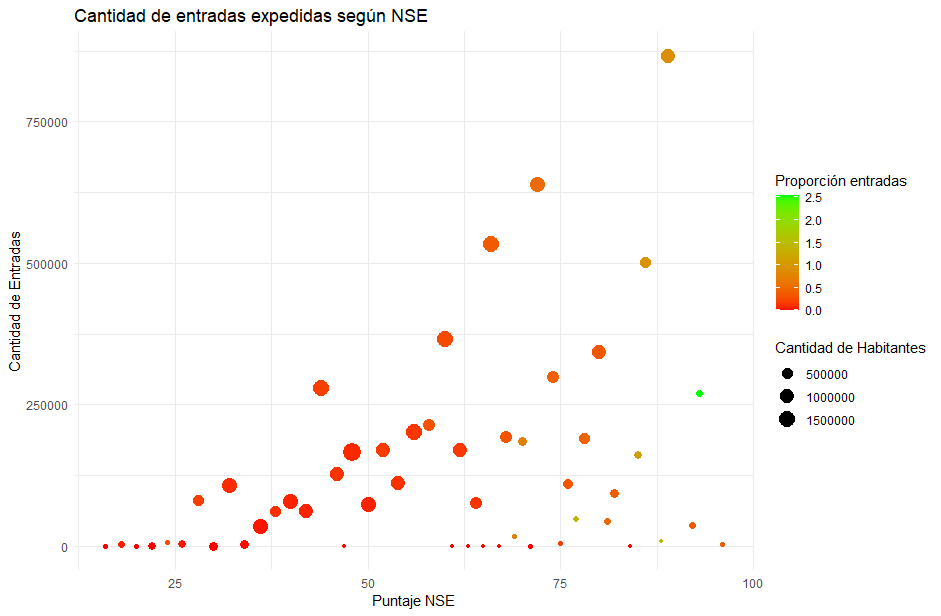
\includegraphics[width=0.9\textwidth]{entradas_nse}
\end{frame}


% Preferencias de museos
\begin{frame}
  \frametitle{Los tipos de museos más concurridos}

    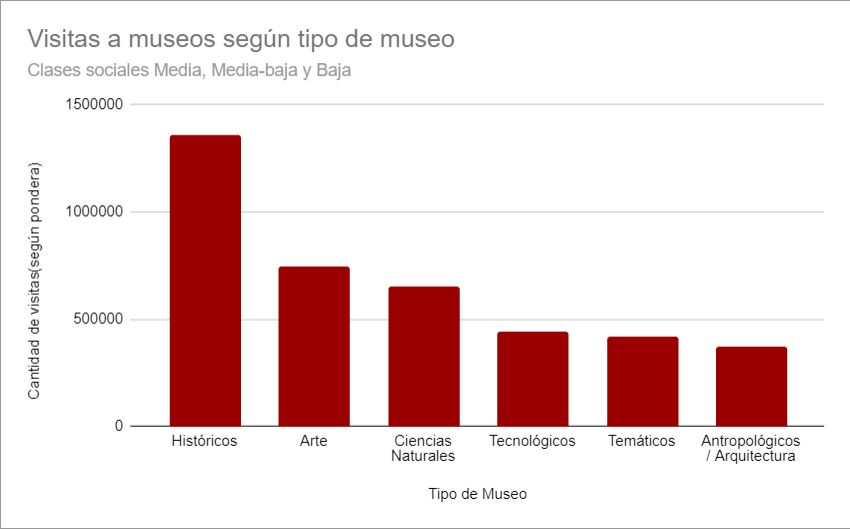
\includegraphics[width=0.95\textwidth]{visitas.jpg}
    Con los datos que se tienen, no es posible saber cuántos museos de cada temática hay en el país.
\end{frame}


% Segmentaciones de consumos culturales y concurrencia a los museos
\begin{frame}
  \frametitle{Comparación de segmentos de consumo cultural}

    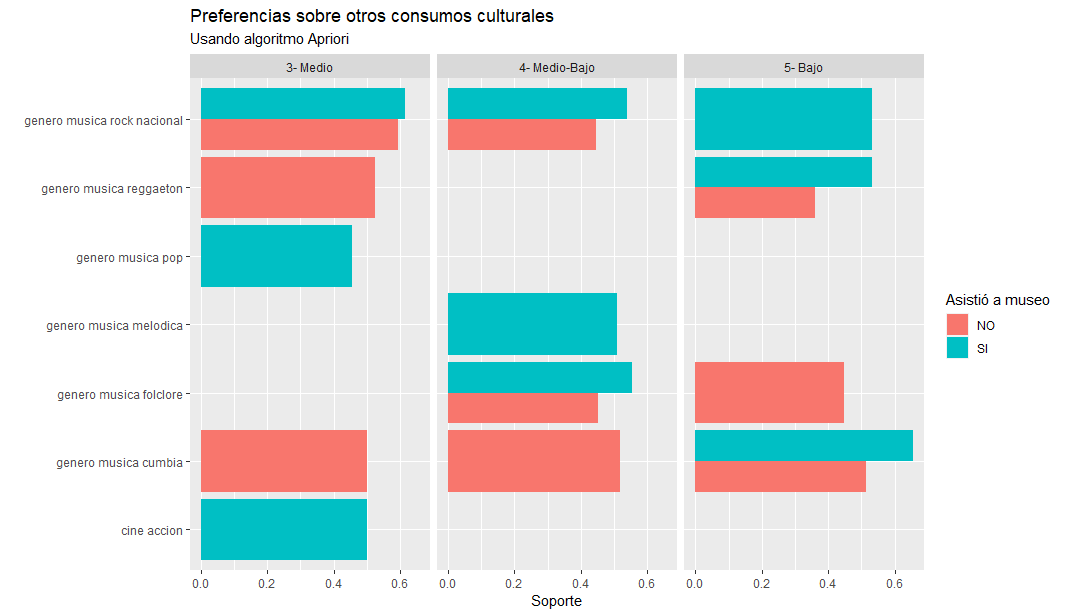
\includegraphics[width=\textwidth]{itemsets.png}
\end{frame}


% Consumos digitales
\begin{frame}
  \frametitle{Cultura digital}
    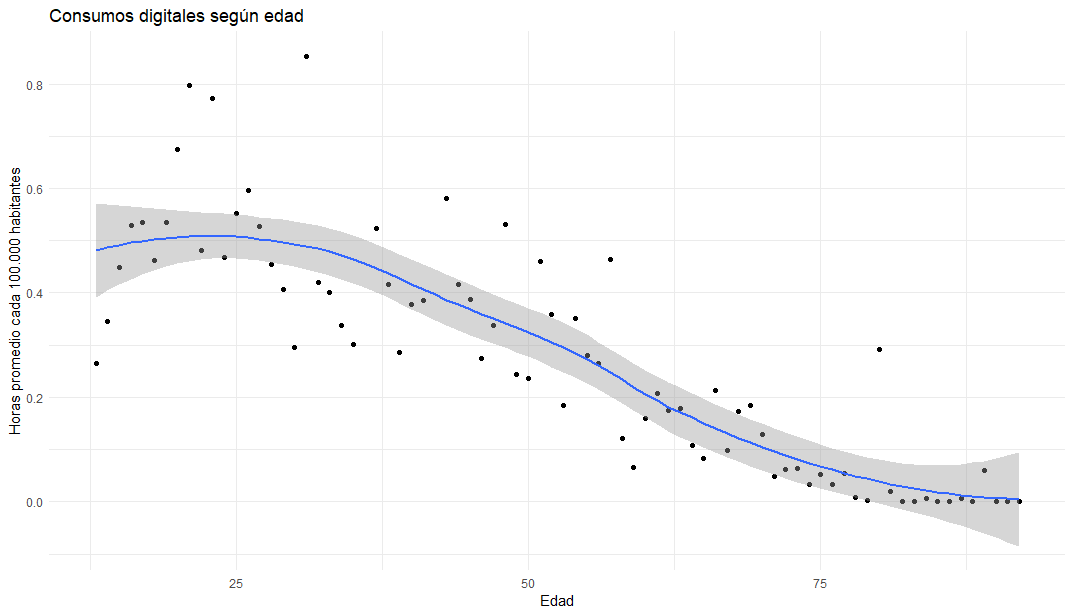
\includegraphics[width=\textwidth]{consumos_digitales.png}
\end{frame}


% Situación PSH
\begin{frame}
  \frametitle{Visitas a museos y situación laboral}
%    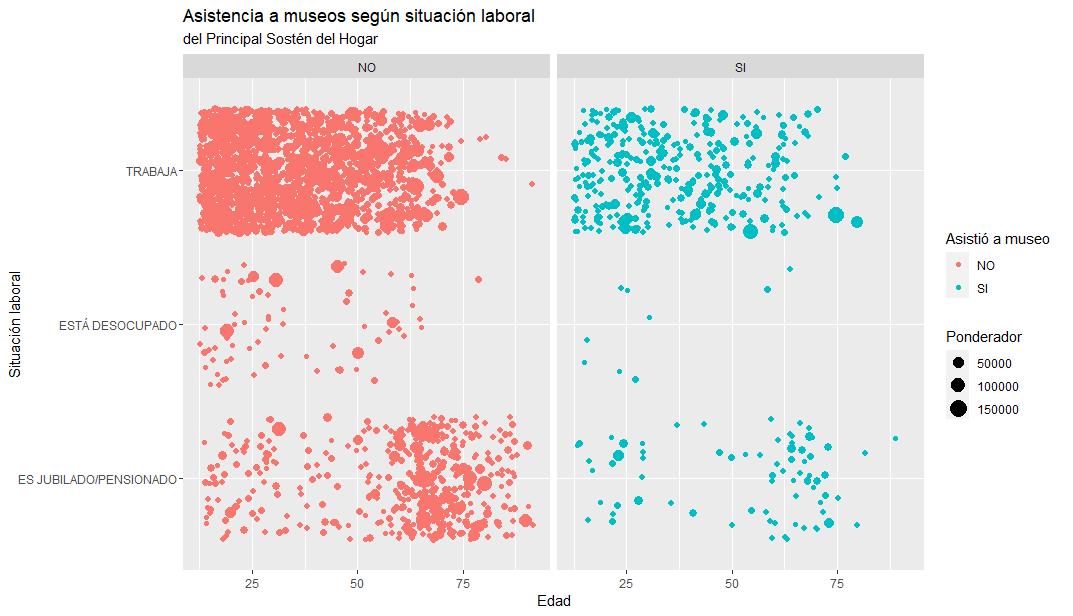
\includegraphics[width=\textwidth]{situacion_psh.png}
    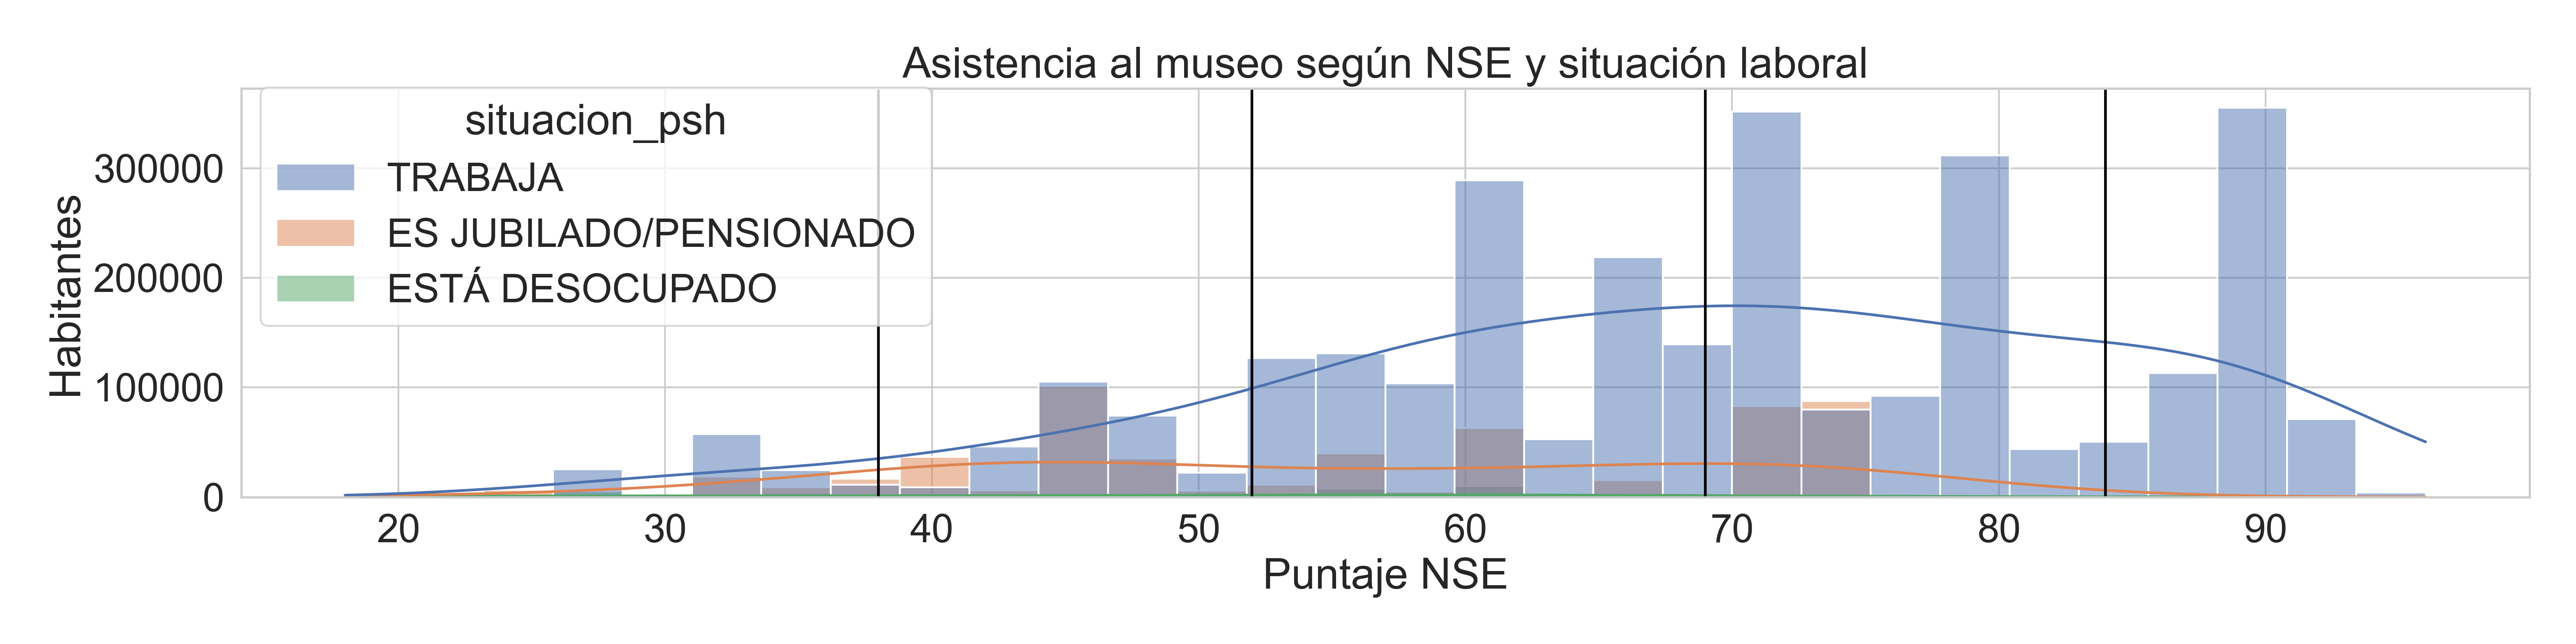
\includegraphics[height=0.32\textheight]{dist_asistentes_lab.png}
    \vfill
    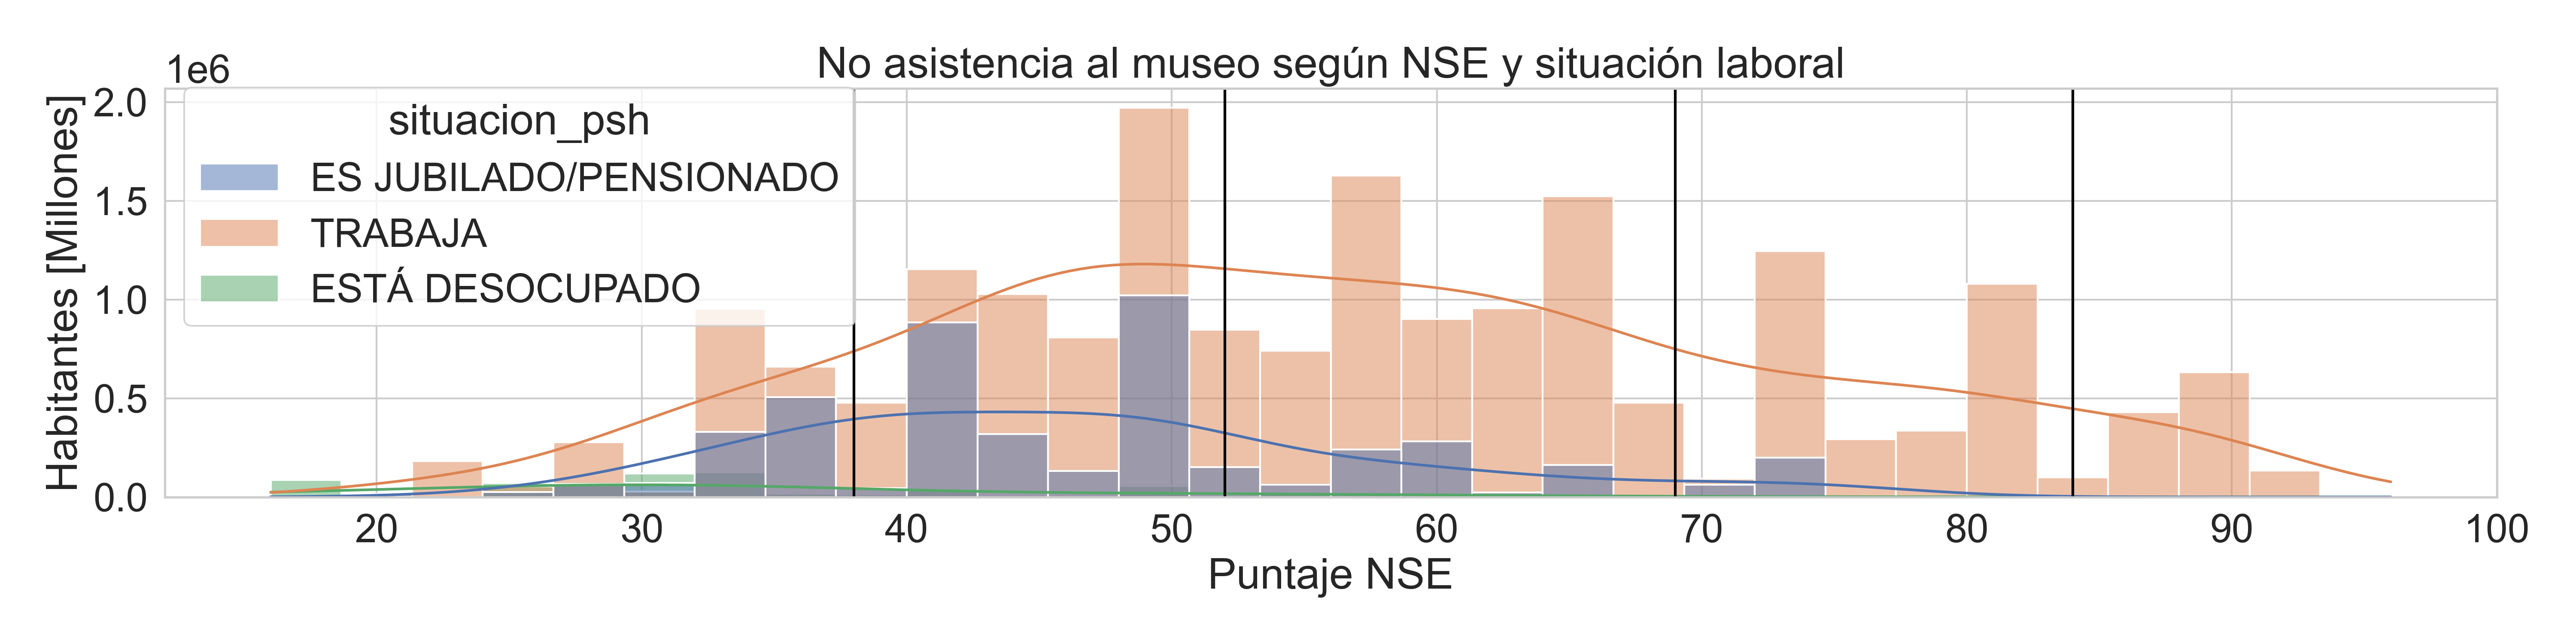
\includegraphics[height=0.32\textheight]{dist_no_asistentes_lab.png}
\end{frame}


% Nivel de estudios
\begin{frame}
  \frametitle{Visitas a museos y escolaridad}

    \begin{columns}
      \column{0.75\textwidth}
        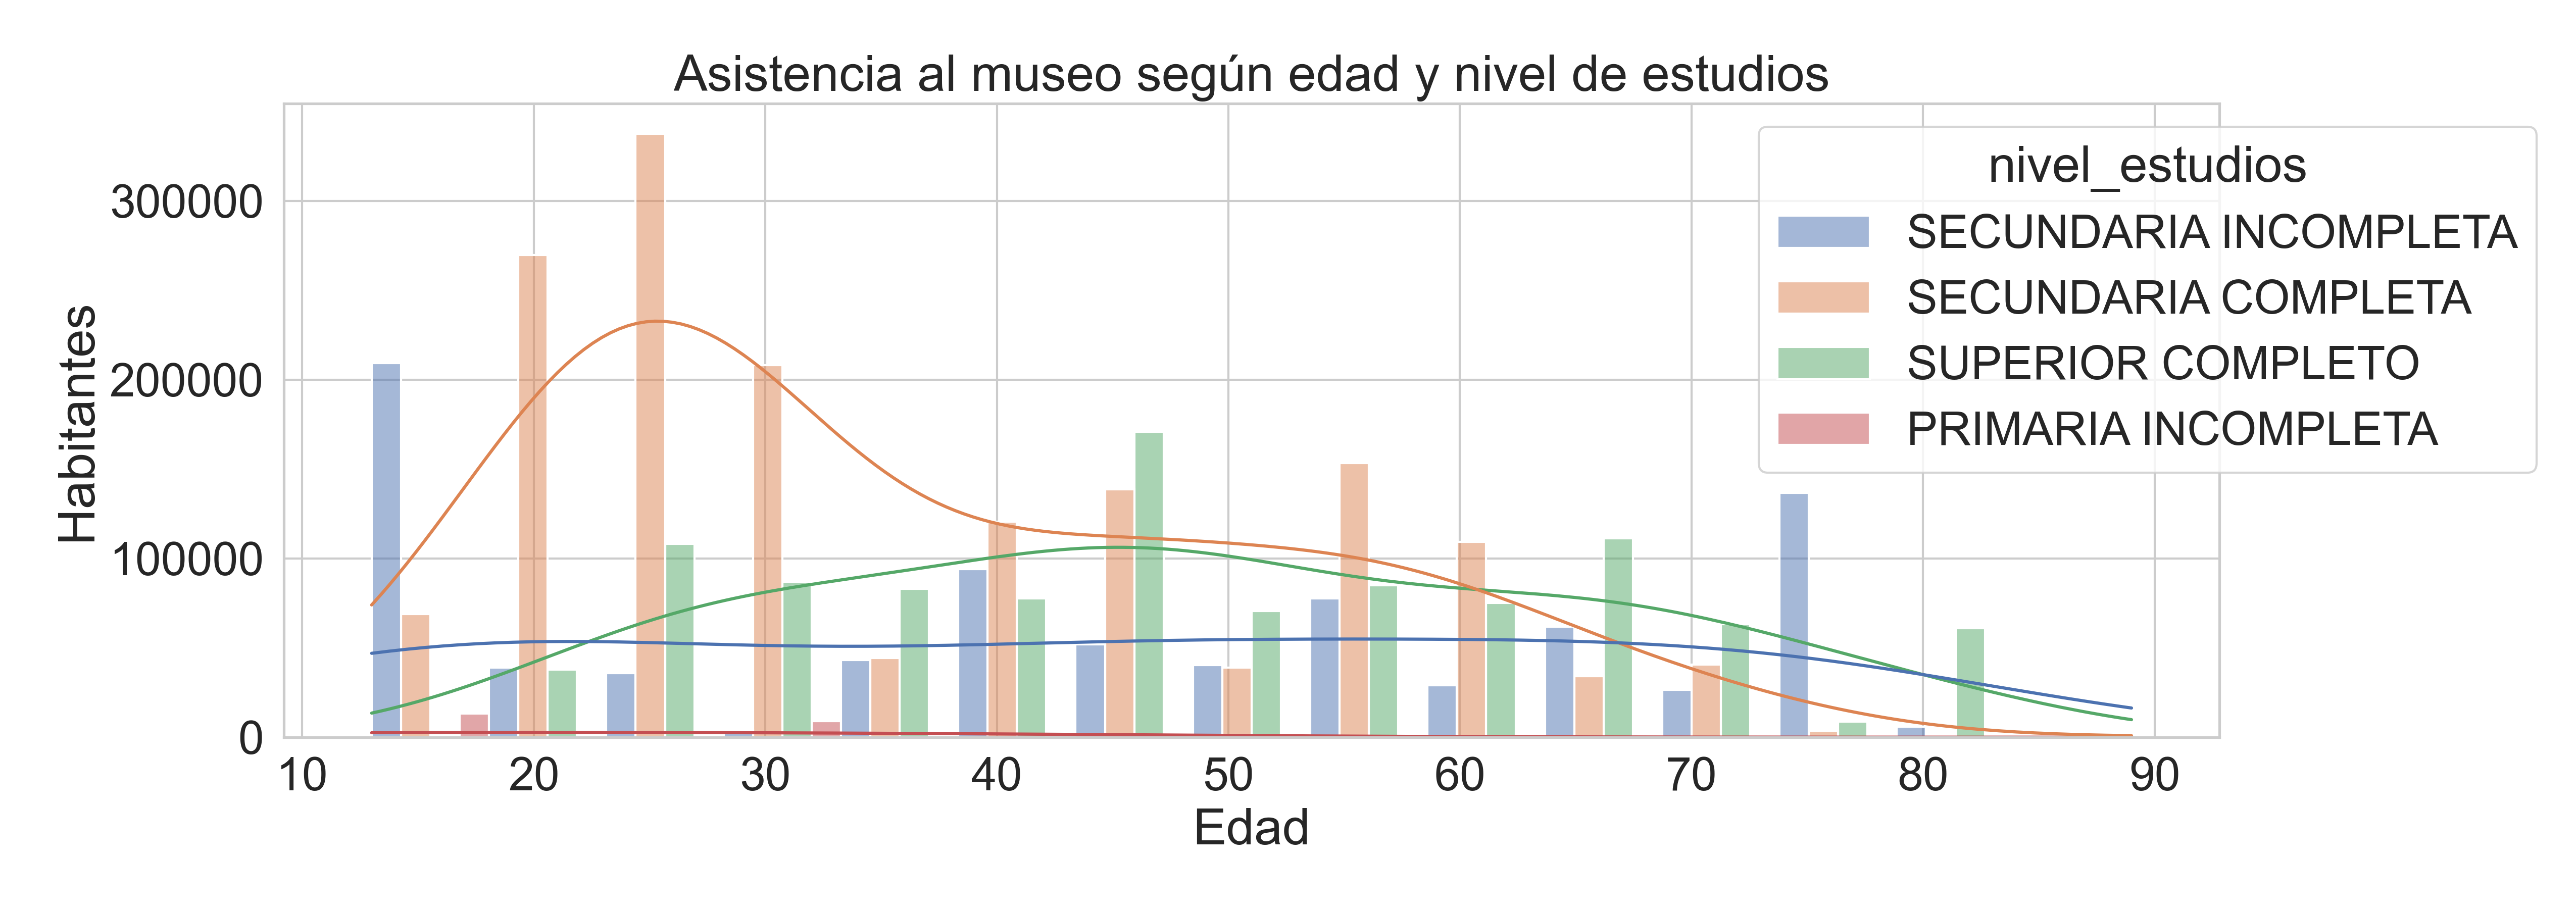
\includegraphics[width=\textwidth]{dist_asistentes.png}
        \vfill
        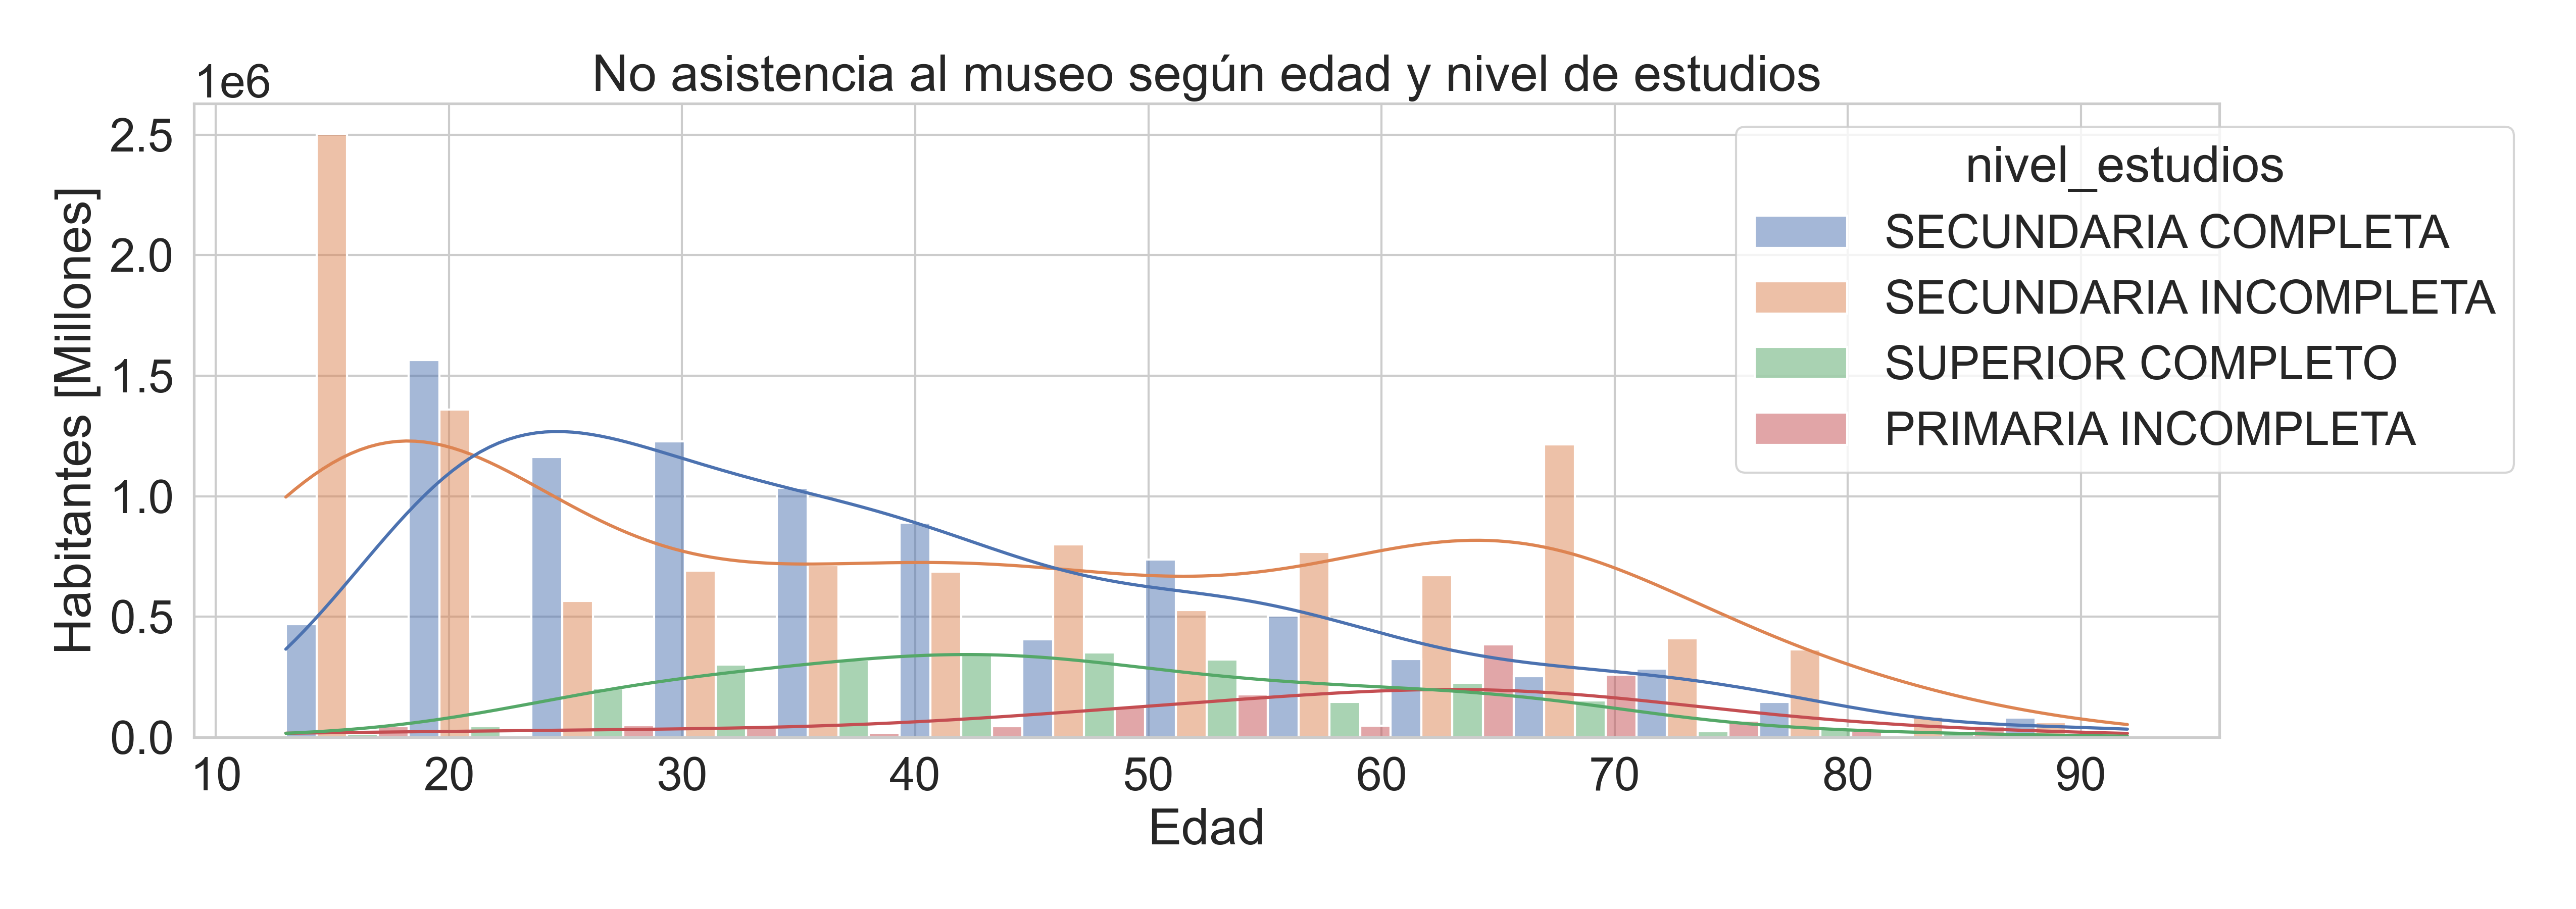
\includegraphics[width=\textwidth]{dist_no_asistentes.png}

      \column{0.25\textwidth}
        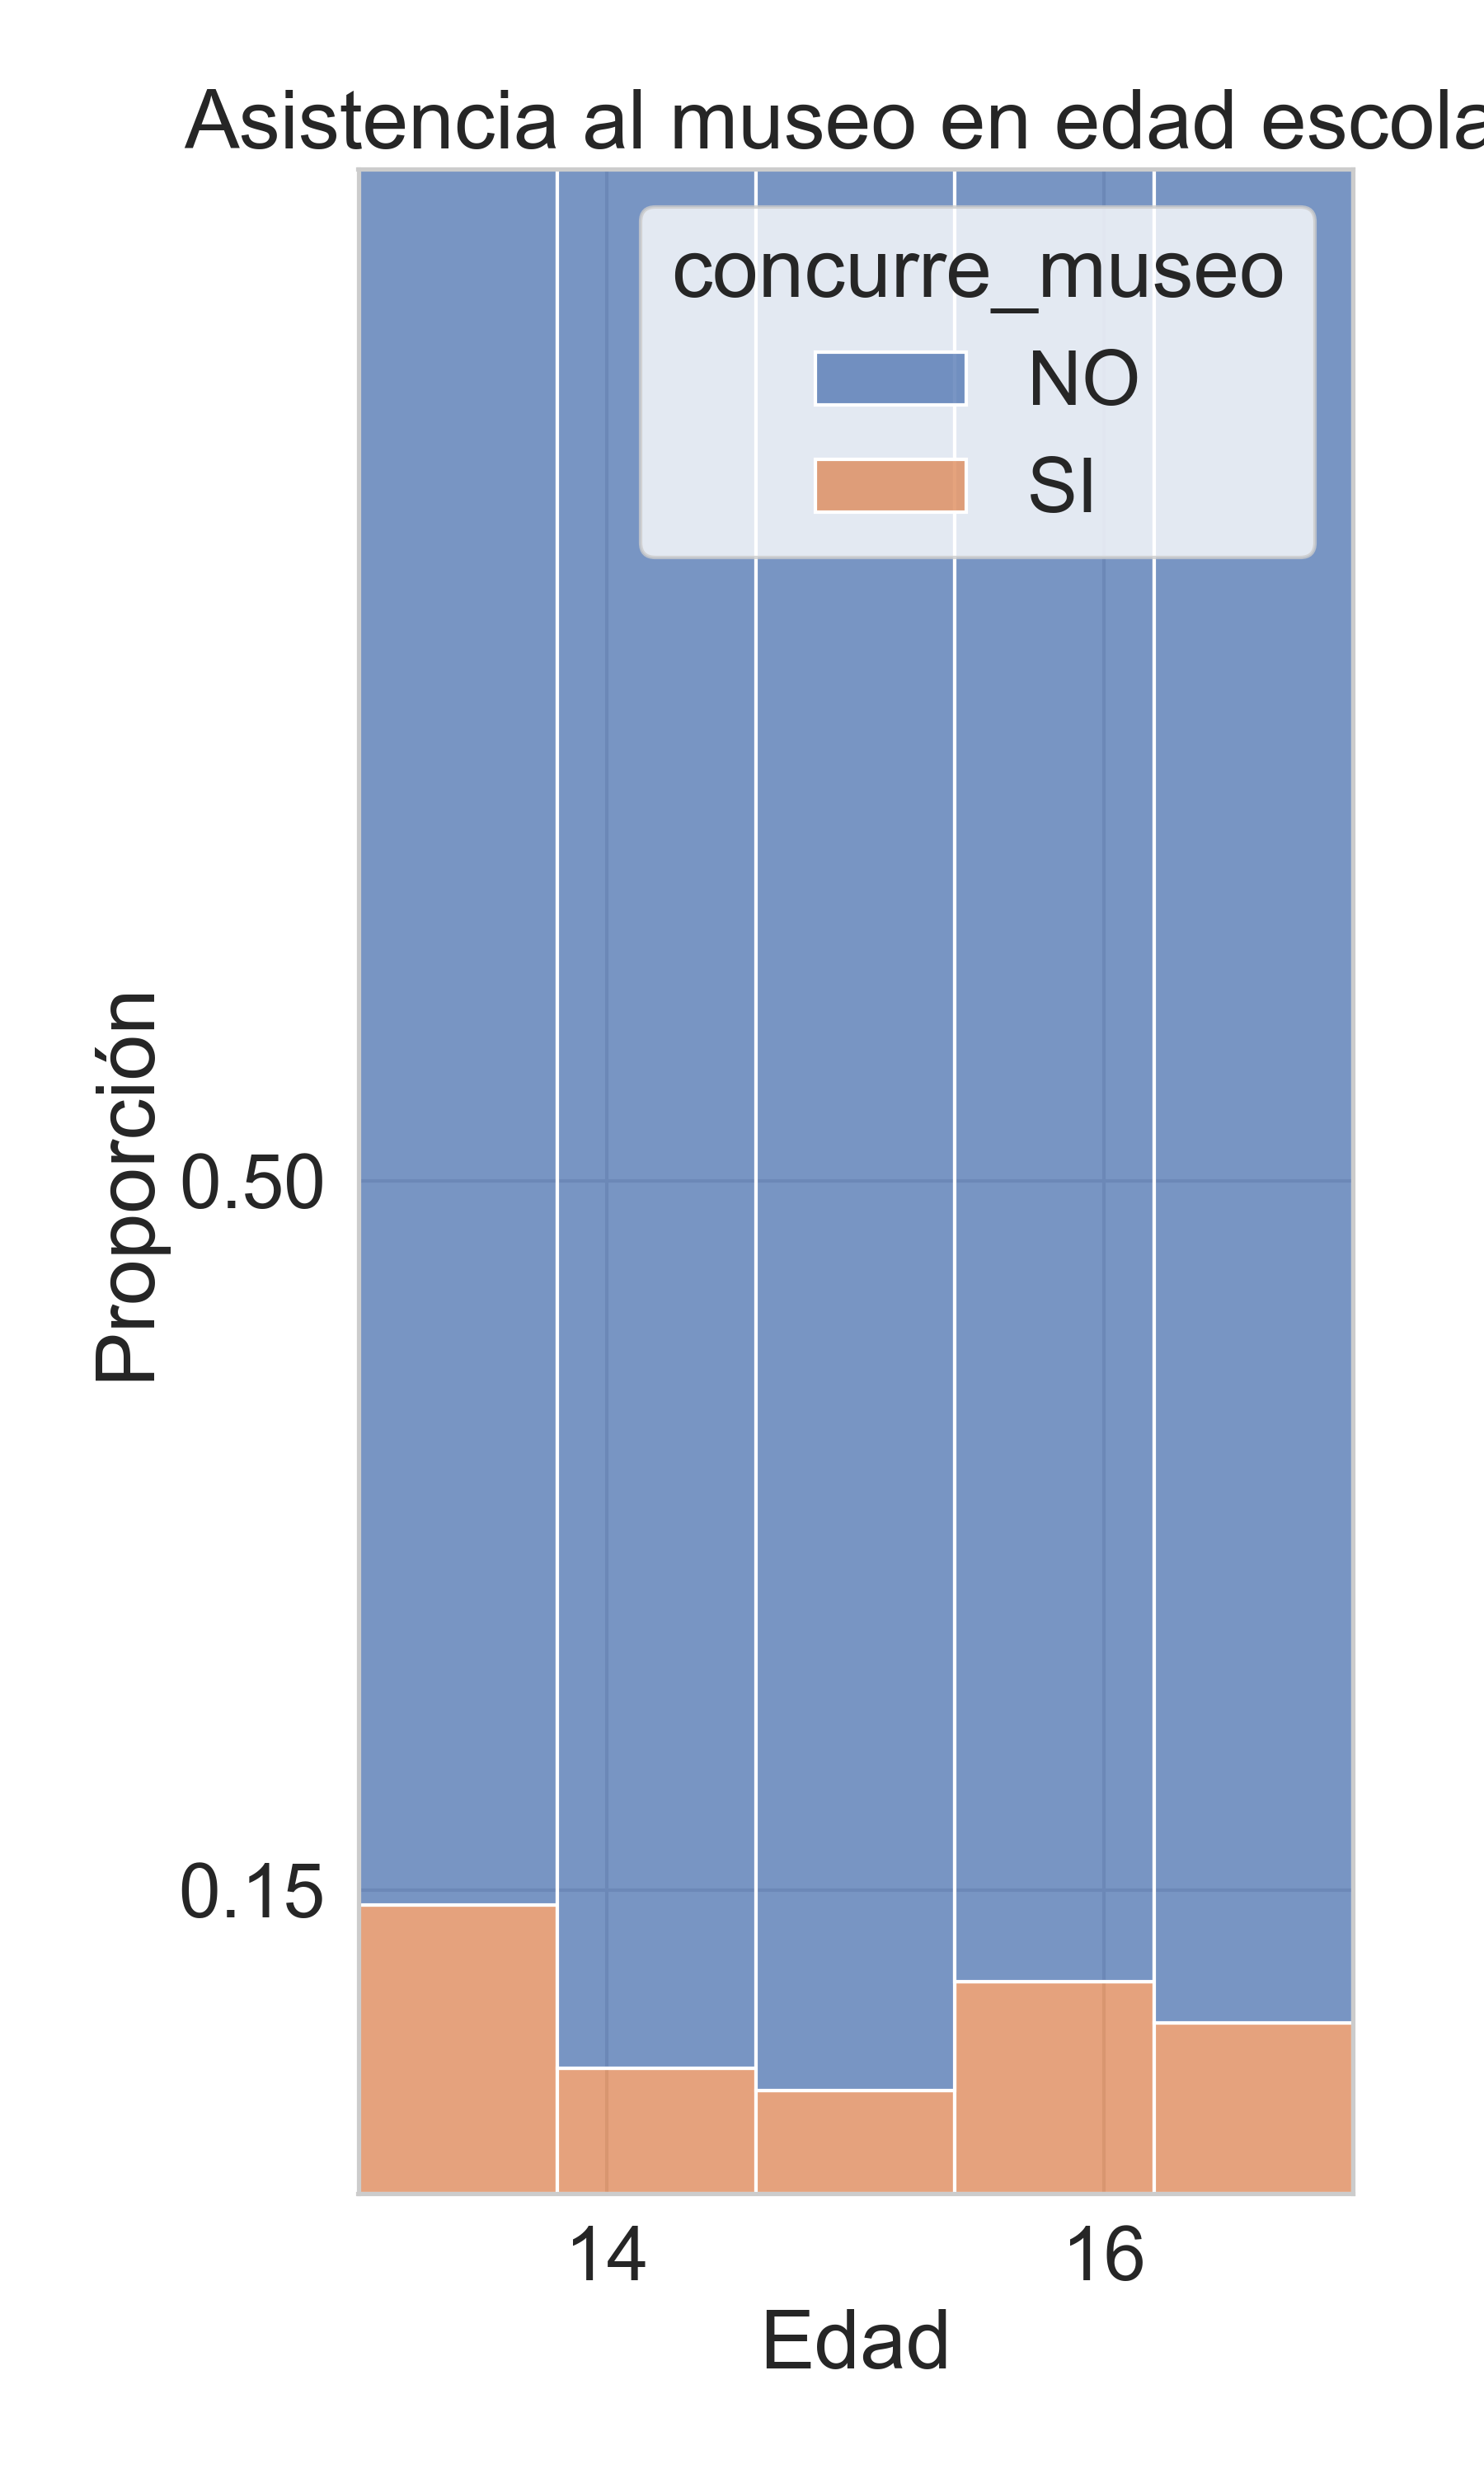
\includegraphics[width=\textwidth]{edad_escolar.png}
    \end{columns}

\end{frame}


% Cantidad de museos y entradas
\begin{frame}
  \frametitle{Modelo de concurrencia al museo}
  \begin{columns}
    \column{0.75\textwidth}
    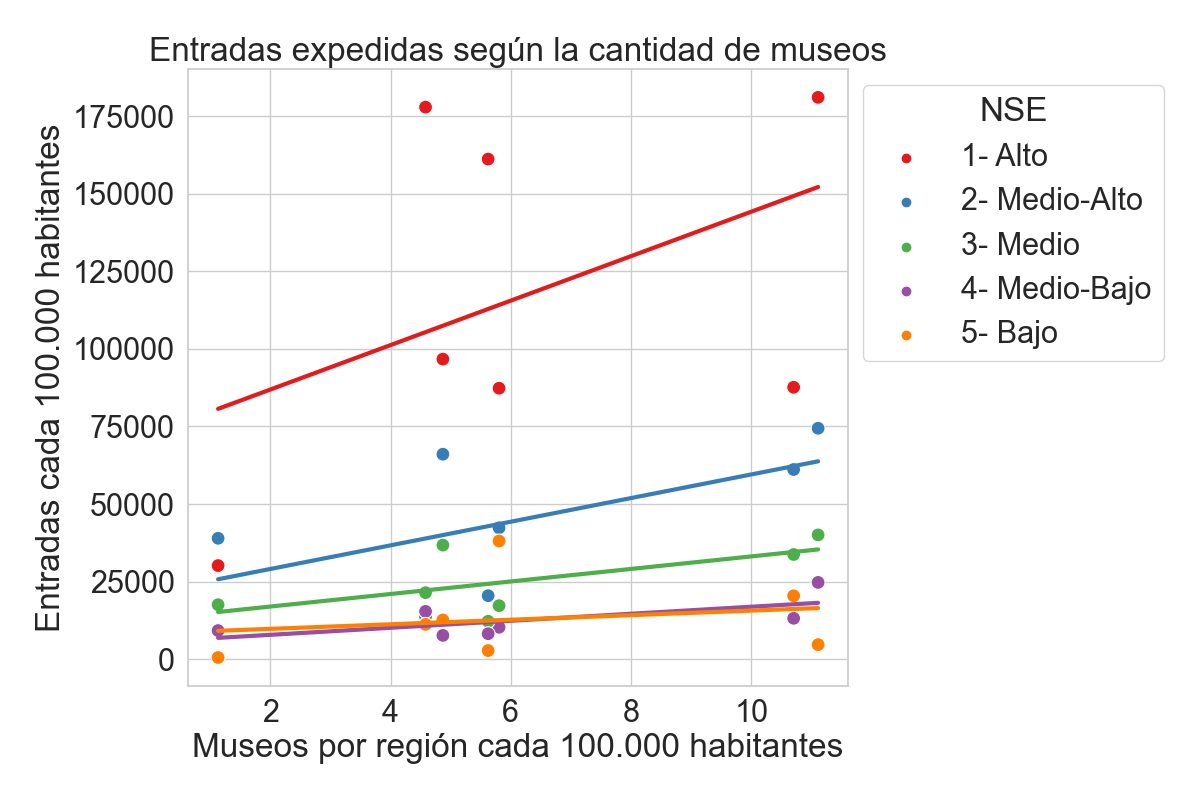
\includegraphics[height=0.9\textheight]{modelo_entrada_museo}
    Multiple R-squared: 0.7544, Adjusted R-squared: 0.6659

    \column{0.25\textwidth}
    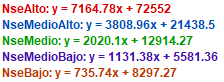
\includegraphics[width=0.9\textwidth]{rectas.png}
  \end{columns}


\end{frame}


% Conclusiones
\begin{frame}
  \frametitle{Conclusiones y trabajo a futuro}
    \begin{itemize}
      \item El contexto socio-económico es muy influyente en la concurrencia a museos.
      \item La encuesta podría indagar en las razones de no concurrencia a museos.
      \item Hay una oportunidad de incrementar la concurrencia con las visitas a museos en edad escolar.
      \item Los consumos culturales tienden a ser más digitales. Los museos pueden tomar la iniciativa.
    \end{itemize}
\end{frame}


% Final
{
  \usebackgroundtemplate{
    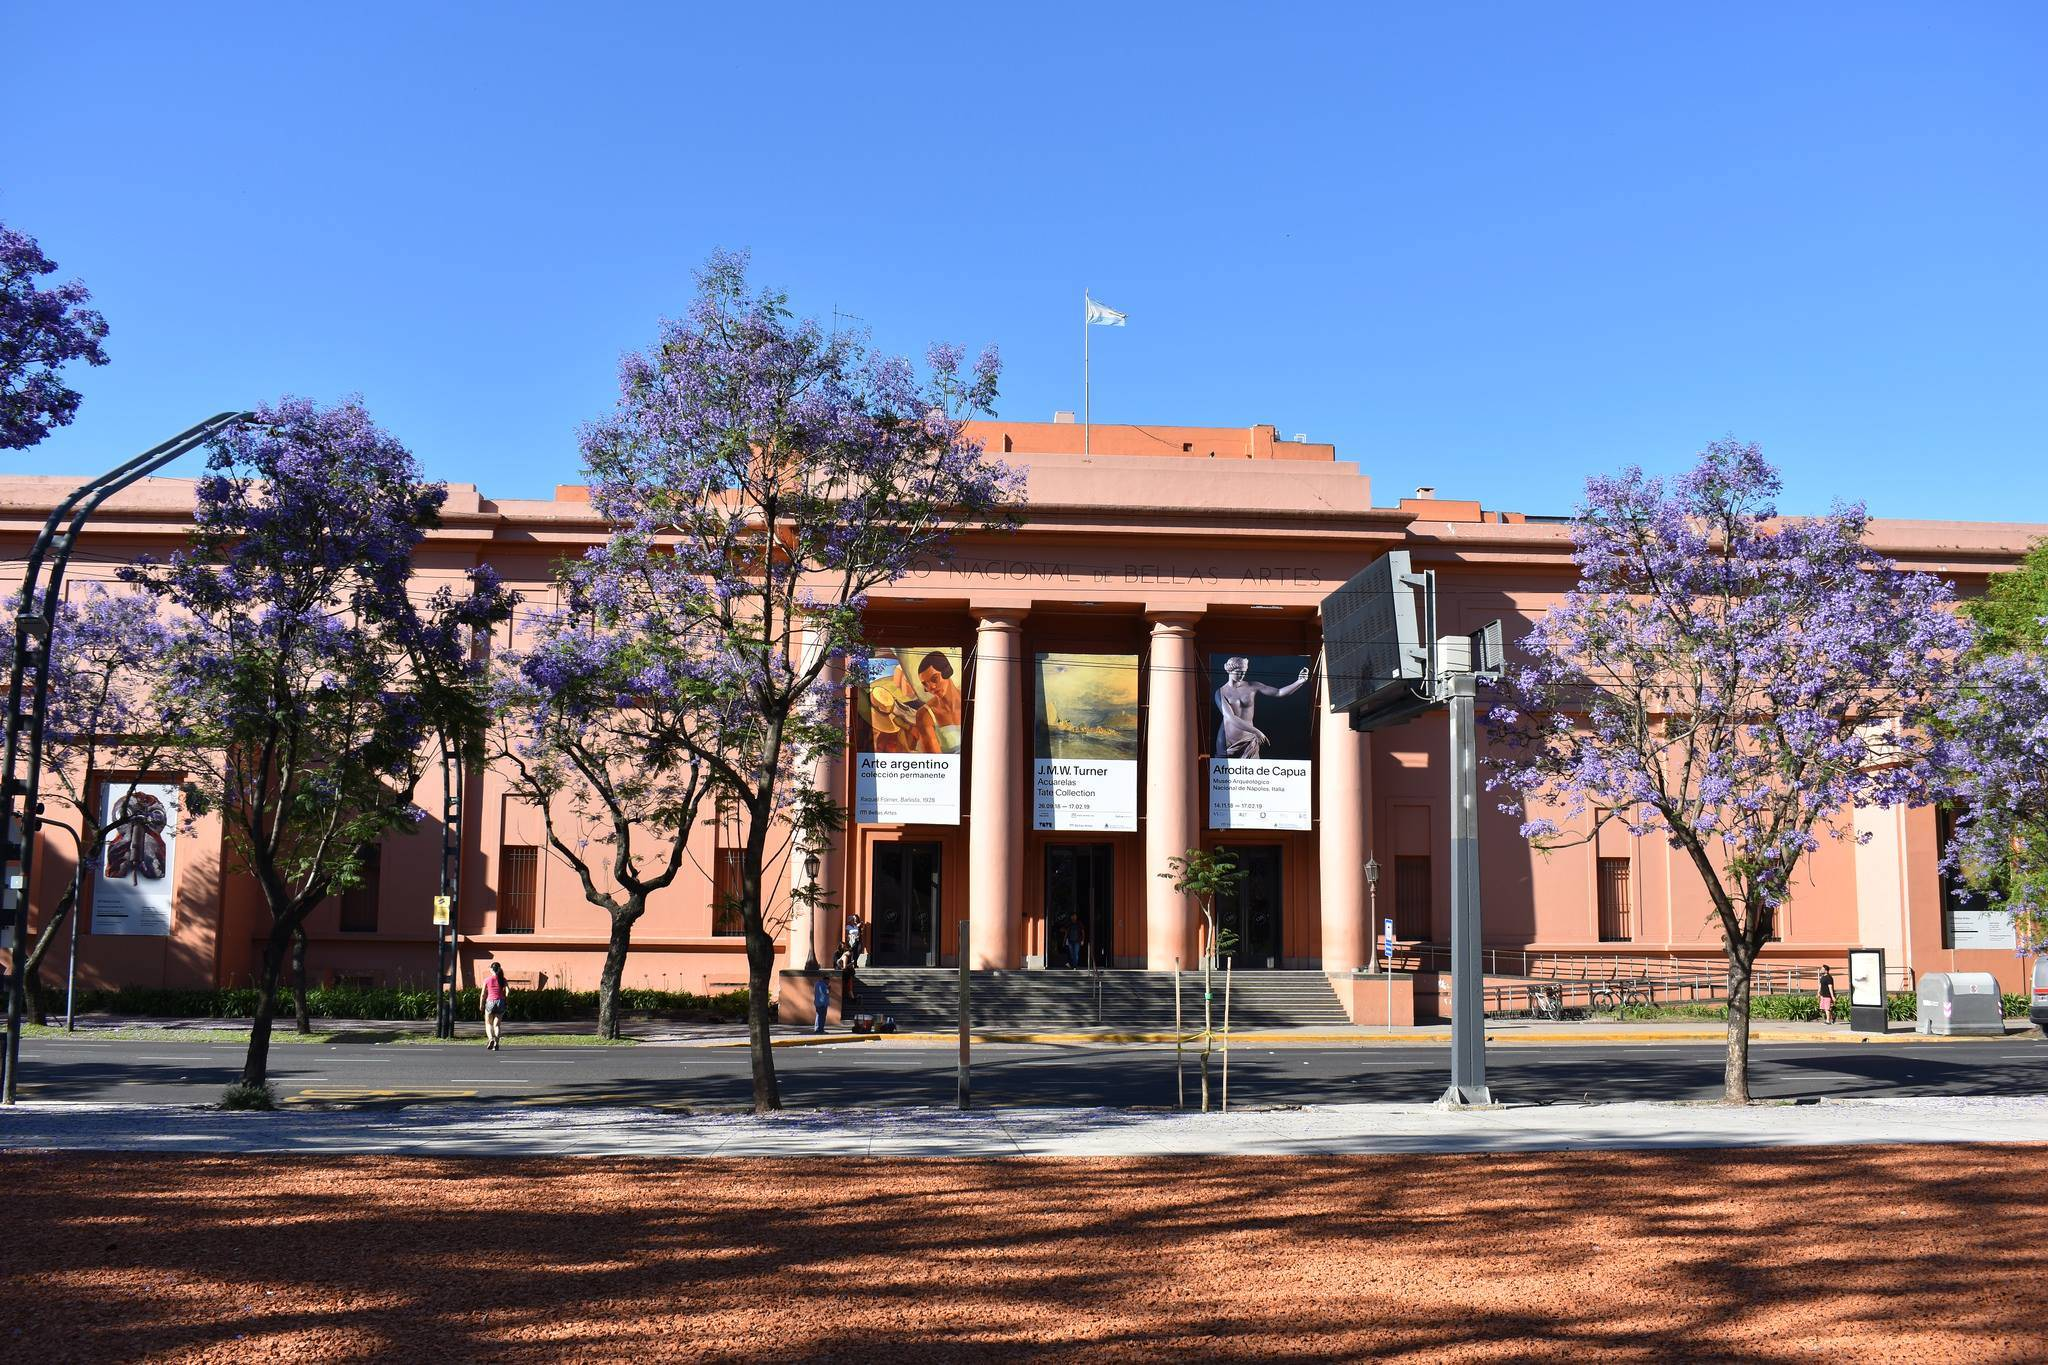
\includegraphics[width=1.2\paperwidth]{mnba-frente.jpg}
  }
  \begin{frame}
    \frametitle{¡Gracias!}

    \vspace{15em}

    \begin{alertblock}{Vayan a los museos}
      ¡Gracias por su atención!\\
      ¿Alguna pregunta?
    \end{alertblock}
  \end{frame}
}


% Fuentes
\begin{frame}
  \frametitle{Fuentes}
  \begin{itemize}
    \item \href{https://datos.cultura.gob.ar/dataset/encuesta-nacional-de-consumos-culturales-2017}{ENCC 2017, Ministerio de Cultura}\\
    \item \href{https://datos.gob.ar/dataset/jgm-servicio-normalizacion-datos-geograficos/archivo/jgm_8.26}{Servicio de Normalización de Datos Geográficos, IGN}
    \item \href{https://datos.gob.ar/dataset/cultura-mapa-cultural-espacios-culturales}{Mapa de Espacios Culturales, Ministerio de Cultura}
  \end{itemize}
  
\end{frame}

% Slide oculta, datos del modelo
\begin{frame}
  \frametitle{Valores del modelo}
\begin{block}{Modelo lineal}
  $entradas\_por\_hab =  museos\_por\_hab \times NSEdenom$
\end{block} 

Residuals:
\resizebox{4cm}{!}{%
  \begin{tabular}{lllll}
  Min    & 1Q    & Media & 3Q   & Max   \\
  -61626 & -9130 & -812  & 5634 & 72512 \\
         &       &       &      &      
  \end{tabular}
}

Coefficients:
\resizebox{\textwidth}{!}{%
  \begin{tabular}{lllll}
                                         &          &            &         &                       \\
                                         & Estimate & Std. Error & t value & Pr(\textgreater{}|t|) \\
  (Intercept)                            & 72552    & 22640      & 3.205   & 0.00367 **            \\
  museos\_por\_hab                       & 7165     & 3204       & 2.236   & 0.03453 *             \\
  NSEdenom2- Medio-Alto                  & -51114   & 32017      & -1.596  & 0.12295               \\
  NSEdenom3- Medio                       & -59638   & 32017      & -1.863  & 0.07430 .             \\
  NSEdenom4- Medio-Bajo                  & -66971   & 32017      & -2.092  & 0.04678 *             \\
  NSEdenom5- Bajo                        & -64255   & 32017      & -2.007  & 0.05569 .             \\
  museos\_por\_hab:NSEdenom2- Medio-Alto & -3356    & 4532       & -0.740  & 0.46590               \\
  museos\_por\_hab:NSEdenom3- Medio      & -5145    & 4532       & -1.135  & 0.26705               \\
  museos\_por\_hab:NSEdenom4- Medio-Bajo & -6033    & 4532       & -1.331  & 0.19510               \\
  museos\_por\_hab:NSEdenom5- Bajo       & -6429    & 4532       & -1.419  & 0.16836              
  \end{tabular}
}


Residual standard error: 27740 on 25 degrees of freedom
Multiple R-squared:  0.7544,	Adjusted R-squared:  0.6659 
F-statistic: 8.531 on 9 and 25 DF,  p-value: 0.00001021
  
\end{frame}


\end{document}
